\section{Results}

\subsection{Descriptive statistics}

The 168,347 patients (who had onset-to-scan of within 255 minutes) attended 118 hospitals with admissions ranging from 358 to 4,559, with thrombolysis rates ranging from 5.9\% to 39.2\%. Of those 133,516 patients that did not receive thrombolysis, their range of disability at discharge was: 12\% mRS 0, 33\% mRS 0-1, 52\% mRS 0-2, 69\% mRS 0-3, 82\% mRS 0-4, and 88\% mRS 0-5 at discharge. Of those 34,831 patients that received thrombolysis, their range of disability at discharge was: 15\% mRS 0, 35\% mRS 0-1, 54\% mRS 0-2, 69\% mRS 0-3, 81\% mRS 0-4, and 86\% mRS 0-5.

Table \ref{tab:descriptive_stats} shows further descriptive statistics for the patients who received thrombolysis.

\begin{minipage}{1\textwidth}
\small
\renewcommand{\arraystretch}{1.2}
\begin{longtable}[]{@{}lllllllll@{}}
\caption{Descriptive statistics for patients who received thrombolysis}\label{tab:descriptive_stats}\\
\toprule
Patient feature &  Mean & Std Dev & Min & Q1 & Q2 & Q3 & Max\tabularnewline
\endhead
\midrule
Age (5 year age bands) & 73 & 13 & 37.5 & 62.5 & 72.5 & 82.5 & 92.5\tabularnewline
Proportion male & 0.55 & - & - & - & - & - & -\tabularnewline
Prior disability (mRS) & 0.8 & 1.2 & 0 & 0 & 0 & 1 & 5\tabularnewline
Stroke severity (NIHSS) & 10.8 & 7.0 & 0 & 5 & 9 & 16 & 42\tabularnewline
Onset to thrombolysis time (minutes) &  163 & 60 & 7 & 120 & 155 & 198 & 720\tabularnewline
Discharge disability (mRS) &  2.6 & 1.9 & 0 & 1 & 2 & 4 & 6\tabularnewline
\bottomrule

\end{longtable}
\normalsize
\end{minipage}

\subsection{Feature selection and proposed causal model}

Using the results from Pearn \textit{el at}. \cite{pearn_are_2024}, we selected 7 features as inputs for the model to predict a patient's likelihood of a good outcome at discharge:

\begin{enumerate}
    \item Prior disability level: Disability level (mRS) before stroke
    \item Stroke severity: Stroke severity (NIHSS) on arrival
    \item Stroke team: Attended hospital
    \item Age: Age (as middle of 5 year age bands)
    \item Onset to thrombolysis time: Time from onset to receiving thrombolysis (minutes). This was set to 9,999 if the patient did not receive thrombolysis.
    \item Atrial fibrillation diagnosis: Patient had a diagnosis of atrial fibrillation (either on arrival or diagnosed during admission)
    \item Precise onset known: Onset time recorded was recorded as being precise time (as opposed to a best estimate)
\end{enumerate}

\begin{figure}[!h]
    \centering%\captionsetup{width=.8\linewidth}%
      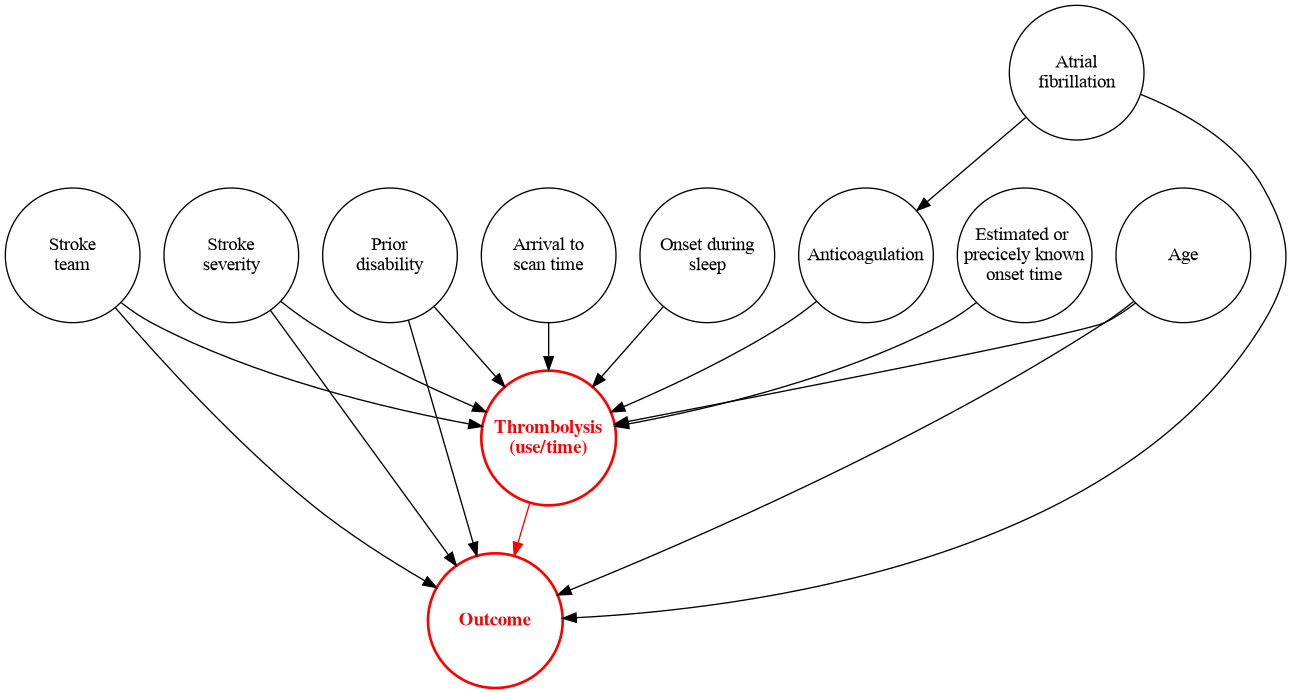
\includegraphics[width=0.80\linewidth]{./images/thrombolysis_dag.png}\\
  \caption{A Directed Acyclic Graph ('DAG') showing the proposed causal relationships. These relationships were derived from feature selection; identifying key features that were predictive of thrombolysis use or outcome. Dashed lines show features affecting propensity to receive thrombolysis; solid lines show features predictive of outcome.}
    \label{fig:single_waterfall_with_ivt}
\end{figure}


\subsection{Model accuracy}

With 7 input features, overall accuracy ranged from 77.6\% to 89.7\% across the six models (standard deviation across the 5 k-folds ranged from 0.001 to 0.002). This represented between 95-98\% of the accuracy that is obtained with all the features as inputs. ROC-AUC ranged from 0.852 to 0.893 across the six models (standard deviation across the 5 k-folds ranged from 0.001 to 0.002). Results were reproducible across the 5 k-folds, so further analysis was performed on the first k-fold split.


\subsection{Individual patient SHAP values}

SHAP values were calculated for each feature for each instance as how each value affects the log odds of having a good outcome at discharge. Figure \ref{fig:single_waterfall_with_ivt} shows a waterfall plot that illustrates the contribution from each feature value on the prediction for whether this individual patient had a good outcome (mRS 0-1) at discharge. This example patient (received thrombolysis at 165 minutes, known precisely, with no prior disability, 72.5 years old, had a moderate stroke, and attended hospital number 103) has a predicted 0.479 log odds (equivalent to 62\% probability) of having a good outcome (mRS 0-1) at discharge. For this patient, the two most influential features (that both increased the likelihood of having a good outcome, mRS 0-1) were prior disability (mRS 0) and onset to thrombolysis time (165 minutes).

\begin{figure}[!h]
    \centering%\captionsetup{width=.8\linewidth}%
      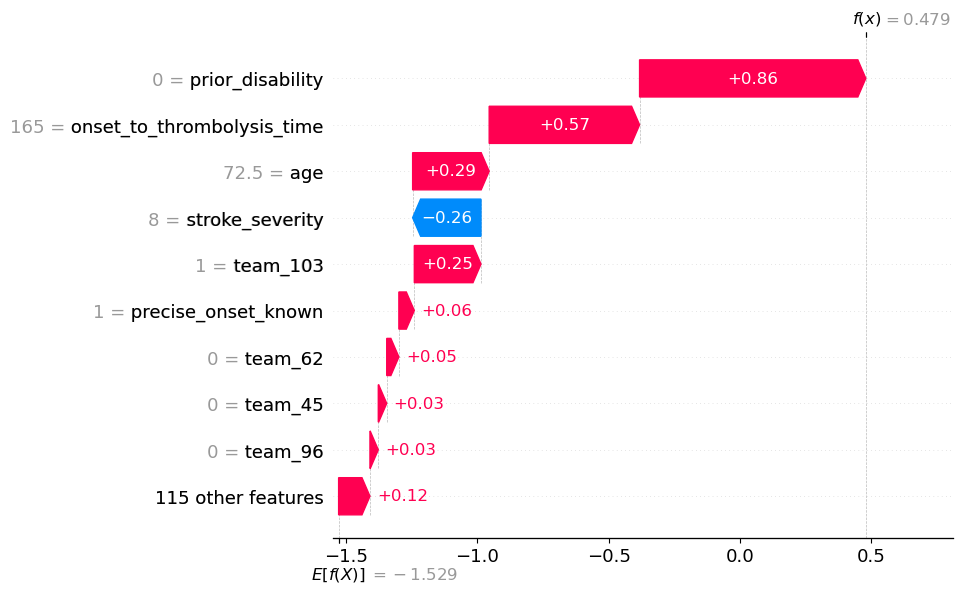
\includegraphics[width=0.95\linewidth]{./images/103_xgb_7_features_1fold_binary_waterfall_plot_patient16_with_IVT.png}\\
  \caption{The waterfall plot for a single patient showing the influence of the nine most influential feature values (y-axis) on the predicted likelihood of having a good outcome (mRS 0-1) on discharge (x-axis). Features are ranked in order of importance (top being most influential), with the contribution from the 10th ranked feature onwards being represented as a single contribution (\textit{115 other features}). The features with name prefix \textit{"team\_"} refers to a stroke team, where the value 1 represents the attended team, and the value 0 represents a team not attended (which may also have a small effect in the model). Each machine learning model applies the same SHAP base value (E[f(X)]) to each patient, this can be interpreted as the most likely outcome given no other knowledge of the instance. The sum of the SHAP base value and the SHAP values for each input feature equates to the overall predicted likelihood of having a good outcome on discharge, shown at the top of the plot (f(x)).}
    \label{fig:single_waterfall_with_ivt}
\end{figure}

\subsection{Global SHAP patterns}

For each patient in the test set we extracted SHAP values for each feature with its corresponding feature value. Figure \ref{fig:global_shap_mrs1} shows the relationship between feature values and the odds of a patient having a good outcome (mRS 0-1) at discharge (a positive SHAP value contributes to an increased likelihood, and a negative SHAP value contributes to a reduced likelihood). We see that low prior disability, lower stroke severity, younger age, receiving thrombolysis (and receiving it sooner after onset), and having no diagnosis of atrial fibrillation contributed to a patient more likely having a good outcome at discharge. Figure \ref{fig:global_shap_ott} focusses on the feature \textit{onset to thrombolysis time}, and its effect at reaching any disability threshold. As time from onset to treatment increased, the beneficial effect of thrombolysis decayed. For thresholds up to, and including, mRS 3, the median effect of thrombolysis remained positive, compared to not receiving thrombolysis, up until the maximum time of 720 minutes. For thresholds of mRS 4 and upwards, the median effect of thrombolysis became negative at longer onset-to-treatment times. This was especially apparent in how thrombolysis changed the overall odds of survival (mRS 0-5) where the median effect of thrombolysis became negative from about 155 minutes. Later thrombolysis may therefore increase the proportion of patients attaining mRS 0-3, but at the cost of some reduction in overall survival. Earlier thrombolysis improved the odds of survival. Figure \ref{fig:global_shap_hosp} shows the contribution from attending a specific hospital to predicting whether the patient had a good outcome at discharge, for each of the mRS threshold levels used to define a good outcome. As the threshold for having a good outcome becomes more inclusive, the range of the effect of the hospital attended had a reduced contribution on the prediction.


%%%%%%%% PUT ON SEPARATE A4 PAGE LANDSCAPE %%%%%%%%%%%

\begin{sidewaysfigure}[!ht]
    \centering
    \begin{subfigure}[b]{0.8\textwidth}
      \centering
      
\includegraphics[trim={0 0 0 1.2cm}, clip, width=1\textwidth]{./images/083_xgb_7_features_5fold_binary_shap_violin_mrs1_0kfold}\\
      \caption{The relationship between feature values and the prediction of whether a patient will have a good outcome (mRS 0-1) at discharge. SHAP base value for this model is -1.529.}
      \label{fig:global_shap_mrs1}
    \end{subfigure}
    \hfill
    \begin{subfigure}[b]{0.8\textwidth}
      \centering    
      
\includegraphics[width=1\textwidth]{./images/083_xgb_7_features_5fold_binary_shap_violin_onset_to_thrombolysis_time_0kfold.jpg}\\
%      
\includegraphics[trim={0 0 0 1.2cm}, clip, width=1\textwidth]{./images/083_xgb_7_features_5fold_binary_shap_violin_ss_0kfold}\\
      \caption{The relationship between onset to thrombolysis time and the prediction of whether a patient will have a good outcome at discharge, for each of the mRS scores used to define a good outcome.}
      \label{fig:global_shap_ott}
    \end{subfigure}
    \hfill
    \begin{subfigure}[b]{0.8\textwidth}
      \centering
      
\includegraphics[trim={0 0 0 1.2cm}, clip, width=1\textwidth]{./images/083_xgb_7_features_5fold_binary_hosp_shap_hist_mrs_0kfold}\\
      \caption{The contribution from attending a specific hospital to predicting whether the patient will have a good outcome at discharge, for each of the mRS scores used to define a good outcome}
      \label{fig:global_shap_hosp}
    \end{subfigure}
    \label{fig:global_shap}
  \caption{The relationship between feature values and SHAP values in predicting whether a patient will have a good outcome. Violin plots show the distribution of SHAP values across the patient population for each feature value, with the mid-line showing the median SHAP value.} 
\end{sidewaysfigure}


\subsection{Counterfactuals (what if patients had not received thrombolysis?)}

\subsubsection{For an individual patient}

Figure \ref{fig:double_waterfall} shows the waterfall plot for a single patient who received thrombolysis (figure \ref{fig:lhs_waterfall_with_ivt}), and its counterfactual case had the same patient not received thrombolysis (figure \ref{fig:rhs_waterfall_without_ivt}). This patient had a predicted 0.479 log odds (62\% probability) of having a good outcome (mRS 0-1) at discharge with thrombolysis, and -0.671 (34\% probability) without thrombolysis. By comparing the log odds contributed by the feature \textit{onset to thrombolysis time} in both cases (when the patient received thrombolysis, and not), we can isolate the predicted direct contribution to a good outcome of being given thrombolysis at a specified duration from stroke onset. For the patient in figure \ref{fig:double_waterfall} the predicted direct contribution to a good outcome (mRS 0-1) for being given thrombolysis at 165 minutes from stroke onset was 0.69 log odds (feature \textit{onset to thrombolysis time} contributed 0.57 log odds to the likelihood of a good outcome when given at 165 minutes, and -0.12 log odds when not given).

\begin{figure}[h]
    \centering
    \begin{subfigure}[t]{0.5\textwidth}
    \centering
    \captionsetup{width=.8\linewidth}%
      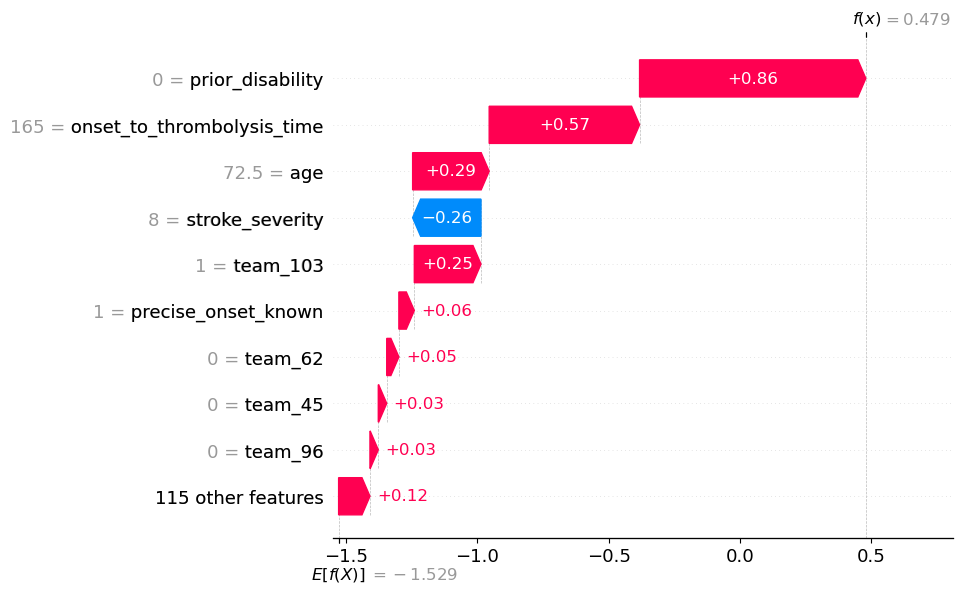
\includegraphics[width=1\linewidth]{./images/103_xgb_7_features_1fold_binary_waterfall_plot_patient16_with_IVT.png}\\
      \caption{Patient with original data (received thrombolysis at 165 minutes)                   
                                                                                }
      \label{fig:lhs_waterfall_with_ivt}
    \end{subfigure}%ults
    \begin{subfigure}[t]{0.5\textwidth}
    \centering
    \captionsetup{width=.8\linewidth}%
      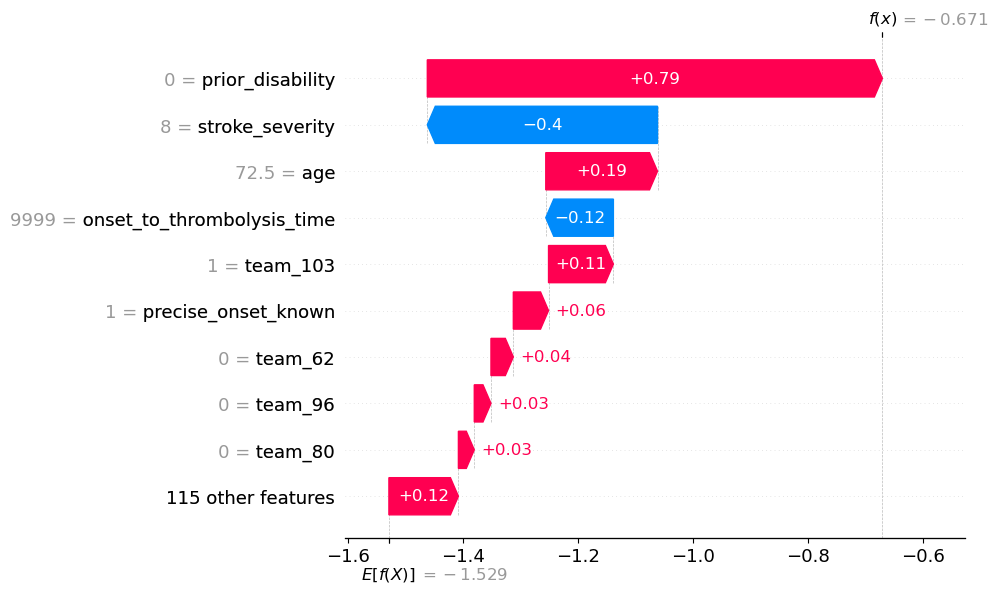
\includegraphics[width=1\linewidth]{./images/103_xgb_7_features_1fold_binary_waterfall_plot_patient16_without_IVT.png}\\
        \caption{Counterfactural case of the same patient not receiving thrombolysis (set onset-to-thrombolysis time to 9999 minutes)}
        \label{fig:rhs_waterfall_without_ivt}
    \end{subfigure}
  \caption{The waterfall plot for a single patient, and its counterfactual case, showing the influence of the nine most influential feature values (y-axis) on the predicted likelihood of having a good outcome (mRS 0-1) on discharge (x-axis). Features are ranked in order of importance (top being most influential), with the contribution from the 10th ranked feature onwards being represented as a single contribution (\textit{115 other features}). The features with name prefix \textit{"team\_"} refers to a stroke team, where the value 1 represents the attended team, and the value 0 represents a team not attended. Each machine learning model applies the same SHAP base value (E[f(X)]) to each patient, this can be interpreted as the most likely outcome given no other knowledge of the instance. The sum of the SHAP base value and the SHAP values for each input feature equates to the overall predicted likelihood of having a good outcome on discharge, shown at the top of the plot (f(x)).}
    \label{fig:double_waterfall}
\end{figure}

\subsubsection{For a cohort of patients}

Using the counterfactual results for all of the patients in the first k-fold test set that received thrombolysis (n = 6,897), figure \ref{fig:probability_shift} shows the shift in predicted probability of a good outcome at discharge, had they not received thrombolysis. For the majority of the cases, there is a greater probability for a good outcome with thrombolysis.

\begin{figure}[!h]
    \centering    \includegraphics[width=0.70\textwidth]%{./images/103_xgb_7_features_1fold_binary_probability_shift_counterfactuals_kfold0_no_max_time_mask}\\
{./images/103_xgb_7_features_1fold_binary_probability_shift_counterfactuals_kfold0_max_time_mask_400}\\

    \caption{The predicted probability of attaining a good outcome with and without thrombolysis, for those patients in the test population that received thrombolysis. Each plot shows the different mRS thresholds used to define a good outcome. The solid black line denotes no change (x=y). The white square shows the same patient across all six plots.}
    \label{fig:probability_shift}
\end{figure}

\subsubsection{The direct contribution of thrombolysis use to the shift in probability of a good outcome}

Using the counterfactual results for all of the patients in the first k-fold test set that received thrombolysis within 300 minutes from stroke onset (n = 6,796), figure \ref{fig:linear_regression_plots} shows a linear regression fitted to the shift in the contribution from receiving thrombolysis towards having a good outcome at discharge (mRS 0-1) with respect to the onset to thrombolysis time. We found, for all treated patients, that the effect of thrombolysis had declined to zero at 328 minutes, and the effect from thrombolysis was improving log odds of a good outcome by 0.90 if it were, theoretically, given at the time of stroke onset. We observed that the maximum theoretical effect of thrombolysis (if given at time of stroke onset) was greater for the severe stroke group (1.048 log odds) than the mild-moderate stroke group (0.771 log odds). However the effect of thrombolysis declined a little faster in the severe stroke group (reaching no effect at 314 minutes for severe stroke patients, compared to 351 minutes for mild-moderate stroke patients). Linear regression coefficients in all three patient groups were statistically significant (table \ref{fig:stats_table_mrs1}). 

\begin{figure}[!ht]
    \centering
    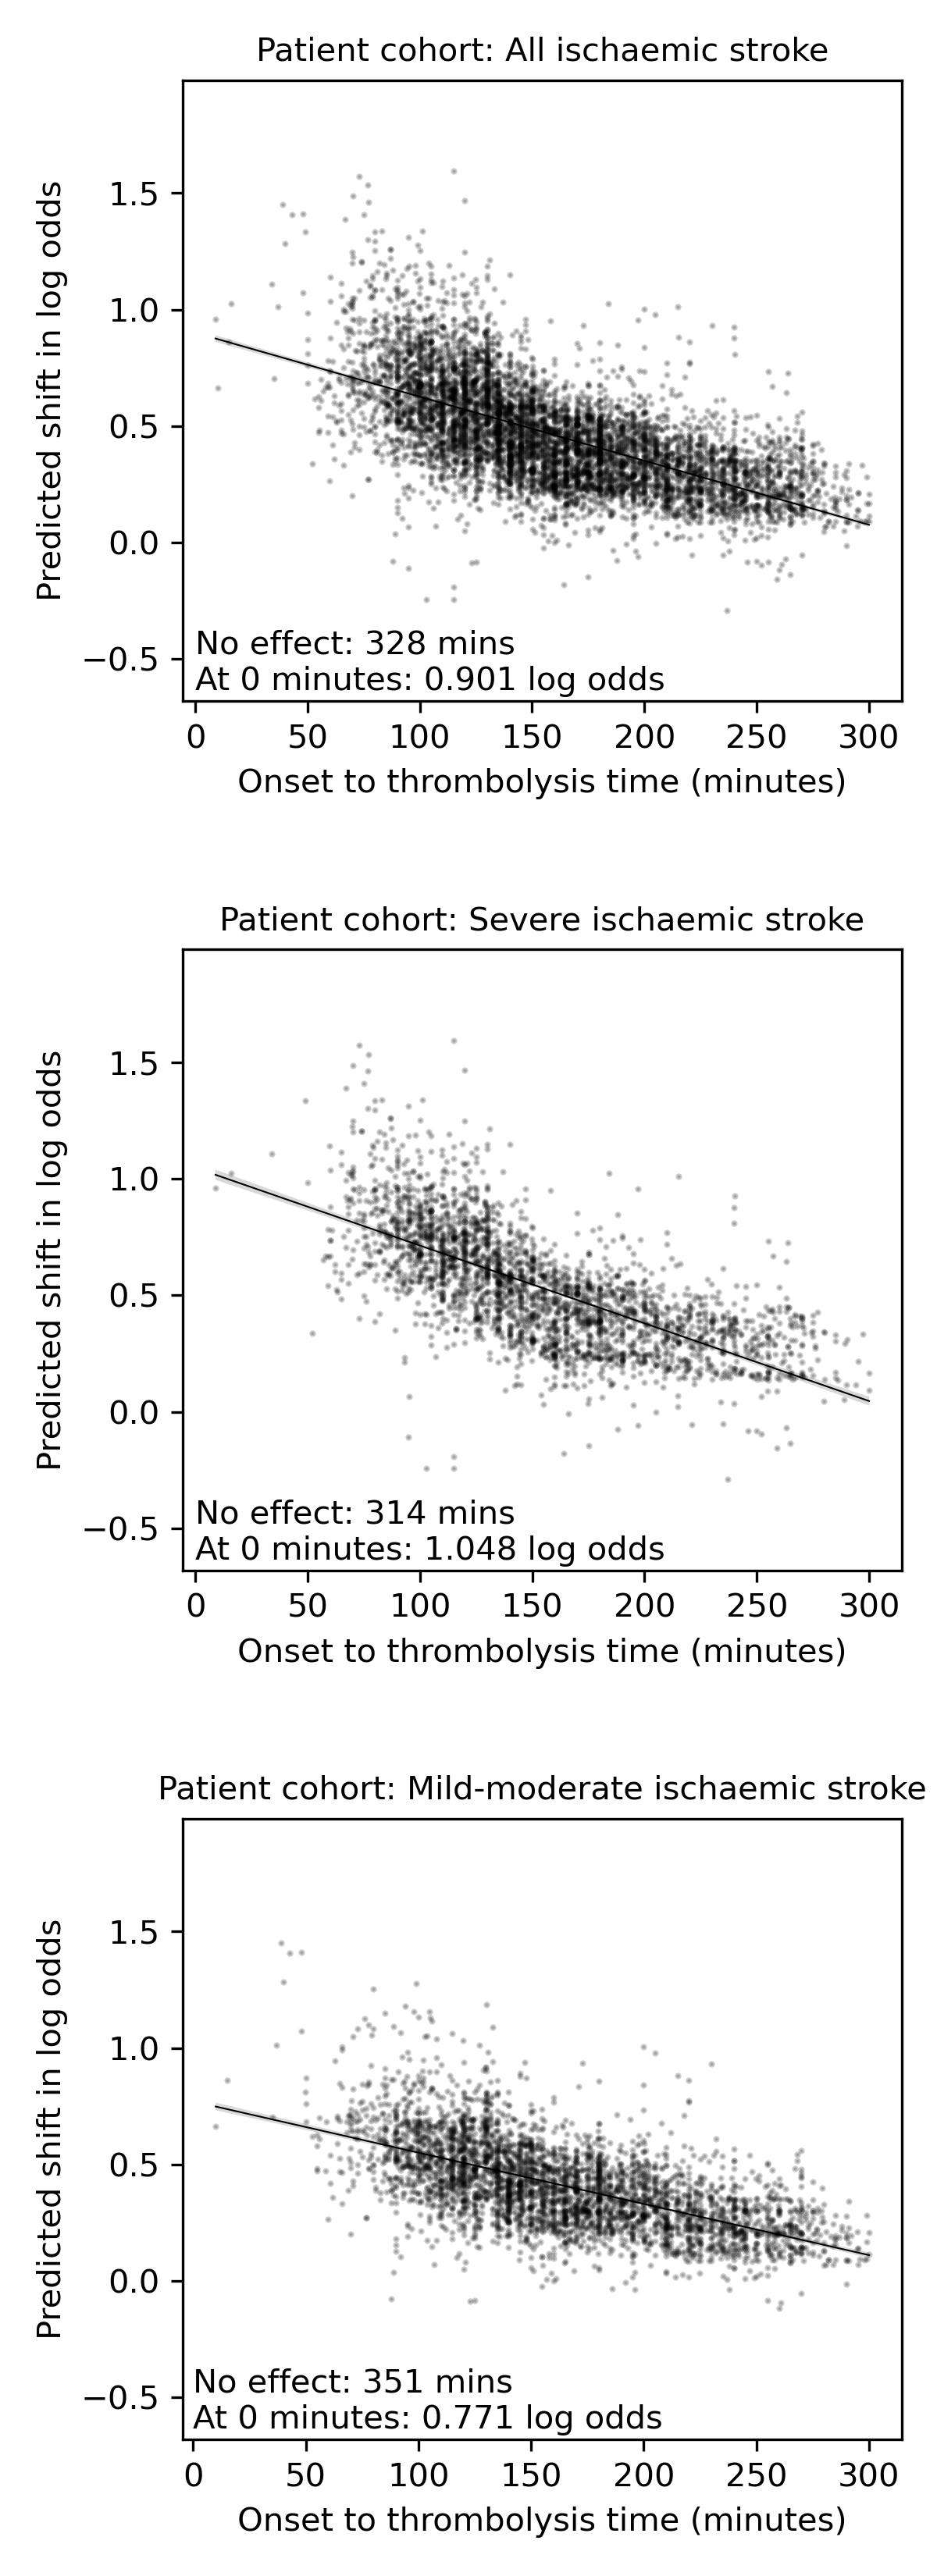
\includegraphics[width=0.50\textwidth]{./images/103_xgb_7_features_1fold_binary_improvement_logodds_mrs0_1_sns_subplots_ivt_shap_paper}\\
    \caption{A linear regression fit to the contribution from receiving thrombolysis on having a good outcome (mRS 0-1) at discharge, with respect to the onset to thrombolysis time (for patients treated within 300 minutes). Top: all treated stroke patients (n = 6,796); Middle: treated severe stroke patients, NIHSS 11+ (n = 2,856); Bottom: treated mild-moderate stroke patients, NIHSS 0-10 (n = 3,940).}
    \label{fig:linear_regression_plots}
\end{figure}


\begin{table}[!ht]
    \caption{Fitting linear regression to the shift in the contribution from receiving thrombolysis towards having a good outcome (mRS 0-1) at discharge with respect to the onset to thrombolysis (OTT) time. Linear regression statistics for different patient cohorts. We used NIHSS 0-10 to define mild-moderate strokes, and NIHSS 11+ to define severe strokes.}
    \centering
        \begin{tabular}{lllllllll}
        \toprule
         Ischaemic stroke type & Variables & coef & std err & t & P$>$$|$t$|$ & [0.025 & 0.975] \\ 
         \midrule
        All & Constant & 0.9012 & 0.007 & 132.519 & 0.000 & 0.888 & 0.915\\
        & OTT time (min) &  -0.0027  & 4.04e-05 & -68.058 & 0.000 & -0.003 & -0.003\\   
        \midrule
        Severe & Constant & 1.0476  &    0.011  & 96.746 & 0.000 & 1.026 & 1.069\\
        & OTT time (mins) & -0.0033 &  6.67e-05  & -50.042 & 0.000 & -0.003 & -0.003\\ 
        \midrule
        Mild-moderate & Constant &           0.7708 &     0.008   & 97.613 & 0.000 & 0.755 & 0.786\\
        & OTT (mins) &  -0.0022 &   4.57e-05 & -48.109 & 0.000 & -0.002 & -0.002\\
        \bottomrule
        \end{tabular}
      \label{fig:stats_table_mrs1}
\end{table}

\FloatBarrier
